\documentclass[11pt,]{article}
\usepackage{lmodern}
\usepackage{amssymb,amsmath}
\usepackage{ifxetex,ifluatex}
\usepackage{fixltx2e} % provides \textsubscript
\ifnum 0\ifxetex 1\fi\ifluatex 1\fi=0 % if pdftex
  \usepackage[T1]{fontenc}
  \usepackage[utf8]{inputenc}
\else % if luatex or xelatex
  \ifxetex
    \usepackage{mathspec}
  \else
    \usepackage{fontspec}
  \fi
  \defaultfontfeatures{Ligatures=TeX,Scale=MatchLowercase}
\fi
% use upquote if available, for straight quotes in verbatim environments
\IfFileExists{upquote.sty}{\usepackage{upquote}}{}
% use microtype if available
\IfFileExists{microtype.sty}{%
\usepackage{microtype}
\UseMicrotypeSet[protrusion]{basicmath} % disable protrusion for tt fonts
}{}
\usepackage[margin=1.0in]{geometry}
\usepackage{hyperref}
\hypersetup{unicode=true,
            pdftitle={Evaluation of machine learning methods for 16S rRNA gene data},
            pdfborder={0 0 0},
            breaklinks=true}
\urlstyle{same}  % don't use monospace font for urls
\usepackage{graphicx,grffile}
\makeatletter
\def\maxwidth{\ifdim\Gin@nat@width>\linewidth\linewidth\else\Gin@nat@width\fi}
\def\maxheight{\ifdim\Gin@nat@height>\textheight\textheight\else\Gin@nat@height\fi}
\makeatother
% Scale images if necessary, so that they will not overflow the page
% margins by default, and it is still possible to overwrite the defaults
% using explicit options in \includegraphics[width, height, ...]{}
\setkeys{Gin}{width=\maxwidth,height=\maxheight,keepaspectratio}
\IfFileExists{parskip.sty}{%
\usepackage{parskip}
}{% else
\setlength{\parindent}{0pt}
\setlength{\parskip}{6pt plus 2pt minus 1pt}
}
\setlength{\emergencystretch}{3em}  % prevent overfull lines
\providecommand{\tightlist}{%
  \setlength{\itemsep}{0pt}\setlength{\parskip}{0pt}}
\setcounter{secnumdepth}{0}
% Redefines (sub)paragraphs to behave more like sections
\ifx\paragraph\undefined\else
\let\oldparagraph\paragraph
\renewcommand{\paragraph}[1]{\oldparagraph{#1}\mbox{}}
\fi
\ifx\subparagraph\undefined\else
\let\oldsubparagraph\subparagraph
\renewcommand{\subparagraph}[1]{\oldsubparagraph{#1}\mbox{}}
\fi

%%% Use protect on footnotes to avoid problems with footnotes in titles
\let\rmarkdownfootnote\footnote%
\def\footnote{\protect\rmarkdownfootnote}

%%% Change title format to be more compact
\usepackage{titling}

% Create subtitle command for use in maketitle
\newcommand{\subtitle}[1]{
  \posttitle{
    \begin{center}\large#1\end{center}
    }
}

\setlength{\droptitle}{-2em}

  \title{\textbf{Evaluation of machine learning methods for 16S rRNA gene data}}
    \pretitle{\vspace{\droptitle}\centering\huge}
  \posttitle{\par}
    \author{}
    \preauthor{}\postauthor{}
    \date{}
    \predate{}\postdate{}
  
\usepackage{booktabs}
\usepackage{longtable}
\usepackage{array}
\usepackage{multirow}
\usepackage[table]{xcolor}
\usepackage{wrapfig}
\usepackage{float}
\usepackage{colortbl}
\usepackage{pdflscape}
\usepackage{tabu}
\usepackage{threeparttable}
\usepackage{threeparttablex}
\usepackage[normalem]{ulem}
\usepackage{makecell}

\usepackage{helvet} % Helvetica font
\renewcommand*\familydefault{\sfdefault} % Use the sans serif version of the font
\usepackage[T1]{fontenc}

\usepackage[none]{hyphenat}

\usepackage{setspace}
\doublespacing
\setlength{\parskip}{1em}

\usepackage{lineno}

\usepackage{pdfpages}
\floatplacement{figure}{H} % Keep the figure up top of the page

\begin{document}
\maketitle

\vspace{35mm}

Running title: Machine learning methods in microbiome studies

\vspace{35mm}

Begüm D. Topçuoğlu\({^1}\), Nick Lesniak\({^1}\), Jenna Wiens\({^2}\),
Mack Ruffin\({^3}\), Patrick D. Schloss\textsuperscript{1\(\dagger\)}

\vspace{40mm}

\(\dagger\) To whom correspondence should be addressed:
\href{mailto:pschloss@umich.edu}{\nolinkurl{pschloss@umich.edu}}

1. Department of Microbiology and Immunology, University of Michigan,
Ann Arbor, MI 48109

2. Department of Computer Science and Engineering, University or
Michigan, Ann Arbor, MI 49109

3. Department of Family Medicine and Community Medicine, Penn State
Hershey Medical Center, Hershey, PA

\newpage

\linenumbers

\subsection{Abstract}\label{abstract}

\newpage

\subsection{Introduction}\label{introduction}

Advances in sequencing technology and decreasing costs of generating 16S
rRNA gene sequences have allowed rapid exploration of human associated
microbiome and its health implications. Currently, the human microbiome
field is growing at an unprecedented rate and as a result, there is an
increasing demand for methods that identify associations between members
of the microbiome and human health. However, this is difficult as human
associated microbial communities are remarkably complex and uneven. It
is unlikely that a single species can explain a disease. Instead,
subsets of those communities, in relation to one another and to their
host, account for the differences in health outcomes. Machine learning
(ML) methods are effective at recognizing and highlighting patterns in
complex microbial datasets. Therefore, researchers have started to
explore the utility of ML models that use microbiota associated
biomarkers to predict human health and to understand the microbial
ecology of diseases such as liver cirrhosis, colorectal cancer,
inflammatory bowel diseases (IBD), obesity, type 2 diabetes and others
(1--11). However, currently the field's use of ML lacks clarity and
consistency on which methods are used and how these methods are
implemented {[}(12); . More notably, flawed ML practices are prevalent
such as using ML pipelines where there is no seperate held-out test
dataset to evaulate model performance, reporting few or only the best
outcomes of different randomizations of cross-validation and showing a
disregard for large differences between cross-validation and testing
performances as well as large confidence intervals of testing
performances (4, 13--19). Moreover, there is a lack of discussion on why
a particular ML model is utilized. Recently, there is a trend towards
using more complex ML models such as random forest, extreme gradient
boosting and neural networks without a discussion on if and how much
model interpretibility is necessary for the study (11, 20--22). The lack
of transparency on modeling methodology and model selection negatively
impact model reproducibility and reliability. We need to strive toward
better machine learning practices by (1) implementing consistent and
reliable machine learning pipelines; (2) selecting ML models that
reflect the goal of the study as it will inform our expectations of
model accuracy, complexity, interpretibility and computational
efficiency.

To showcase a reliable ML pipeline and to shed light on how much ML
model selection can affect modeling results, we performed an empirical
analysis comparing several different ML models using the same dataset
and with a robust ML pipeline. We used a previously published colorectal
cancer (CRC) study (3) which had fecal 16S rRNA gene sequences from 490
patients. We built ML models using fecal 16S rRNA gene sequences to
predict patients with normal colons or patients with colonic tumors
which are called screen relevant neoplasias (SRN). The study had 261
normal and 229 SRN samples. We established modeling pipelines for
L2-regularized logistic regression, L1 and L2 support vector machines
(SVM) with linear and radial basis function kernels, a decision tree,
random forest and XGBoost. Our ML pipeline utilized held-out test data
to evaluate generalization and prediction performance of each ML model.
The median test AUROC varied from 0.601 to 0.695. Random forest had the
highest median AUROC for detecting SRN. Despite the simplicity, the
L2-regularized logistic regression followed random forest in
performance. In terms of computational efficiency, L2 logistic
regression trained the fastest (0.202 hours, std ± 0.019), while XGBoost
took the longest (162.843 hours, std ± 3.986). We found that median
cross-validation and testing AUROC varied only 0.021, which highlights
the importance of a seperate held-out test set and consistent
preprocessing of the data prior to evaluation. Aside from evaluating
generalization and classification performances for each of these models,
this study established standards for modeling pipelines of
microbiome-associated machine learning models.

\subsection{Results}\label{results}

\textbf{Model selection and pipeline construction}

We used a cohort of 490 patients with 261 cases of SRN. For each
patient, we had 6920 features (fecal bacterial abundances) and a
two-class label that defines their colonic health (SRN or normal). All
the cases were independently labeled through colonoscopies. We
established modeling pipelines for a binary prediction task with
L2-regularized logistic regression, L1 and L2 support vector machines
(SVM) with linear and radial basis function kernels, a decision tree,
random forest and extreme gradient boosted decision tree (XGBoost) to
emphasize the differences in model accuracy, complexity,
interpretibility and computational efficiency due to model selection.

For regularized logistic regression and SVM with linear kernel we used
L2 regularization to keep all potentially important features. For
comparison, we also trained an L1 regularized SVM model with linear
kernel. L1-regularization on microbiome data lead to a sparser solution
(i.e., force many coefficients to zero), removing features that could be
correlated with other important features, making it more difficult
include the relationships between the microbes and possibly dropping
features that are important in detecting SRNs. Finally, to explore the
potential for non-linear relationships among features and the outcome of
interest, we trained tree based models, decision tree, random forest and
XGboost, as well as an SVM with non-linear kernel.

We established a robust and reliable ML pipeline where we train and
validate each of the seven models {[}Figure 1{]}. We randomly split the
data into training/validation and test sets so that the
training/validation set consisted of 80\% of the full dataset while the
test set was composed of the remaining data {[}Figure 1{]}. Since the
cases are not uniformly represented in the data, the initial data-split
was stratified to maintain the overall label distribution on both the
training/validation and test sets. Training/validation set consisted of
393 patients (209 SRN), while the test set was composed of 97 patients
(52 SRN). The training/validation data was used for training purposes
and validation of hyperparameter selection, and the test set was used
for evaluation purposes. Validation of hyperparameter selection was
performed using 100 randomizations of five-fold cross-validation on the
training/validation set {[}Figure 1{]}. Similar to the initial
data-split, five-fold cross-validation was also stratified to maintain
the overall label distribution on the training and validation sets. We
validated the cross-validation performances of each hyperparameter
setting over the 100 randomizations and selected the best performing
hyper-parameter setting to train the full training/validation dataset
{[}Figures S1 and S2{]}. We then used the held-out test set to evaluate
the prediction performance of each ML model. The data-split,
hyperparameter selection, training and testing steps were repeated 100
times to get a reliable and robust reading of model prediction
performance {[}Figure 1{]}.

\textbf{Model performance and generalizability.}

We evaluated the prediction performances of seven binary classification
models when applied to held-out test data using the area under the
receiver operating characteristic curve (AUROC) as the discriminative
performance metric. Random forest had significantly higher test AUROC
values than the other models for detecting SRNs. The median AUROC of
random forest was 0.695 (IQR 0.044). L2 logistic regression, XGBoost, L2
SVM with linear and radial basis function kernel AUROC values were not
significantly different from one another. They had median AUROC values
of 0.68 (IQR 0.055), 0.679 (IQR 0.053), 0.678 (IQR 0.056) and 0.668 (IQR
0.056) respectively. L1 SVM with linear kernel and decision tree had
significantly lower AUROC values than the other ML models with median
AUROC of 0.65 (IQR 0.066) and 0.601 (IQR 0.059), respectively {[}Figure
2{]}.

We evaluated the generalization performance of each ML model by
comparing their median cross-validation AUROC and median testing AUROC.
This difference should be low to suggest the model is not overfitting
despite the large number of features. The largest difference between the
two was 0.021 in L1 SVM with linear kernel followed by SVM with radial
basis function kernel and decision tree with a difference of 0.007 and
0.006, respectively {[}Figure 2{]}.

\textbf{Interpretation of each ML model.}

The ML models we built using L2-regularized logistic regression, L1 and
L2 support vector machines (SVM) with linear and radial basis function
kernels, a decision tree, random forest and XGBoost increase in
complexity as they decrase in interpretibility. We interpreted L1 and L2
SVM with linear kernel using the feature weights and L2 logistic
regression using regression coefficients of the trained models. We
examined the 5 predictive (highest weight) and protective (lowest
weight) features identified by the model. We calculated the mean weights
and coefficients of these features over the 100 data-splits. In the
three linear models, OTUs that had the largest mean weights and drove
the detection of SRNs belong to family \emph{Lachnospiraceae}, and
\emph{Ruminococcaceae} (OTU01239, OTU00659, OTU00742, OTU00012,
OTU00050, OTU00015, OTU00768, OTU00822, OTU00609, OTU01212, OTU00629)
and genera \emph{Gamella} (OTU00426) {[}Figure 3{]}. We explained the
feature importances in non-linear models using permutation importance on
the held-out test data. For the tree-based models, permuting
\emph{Peptostreptococcus} (OTU00367) abundances randomly, dropped the
predictive performances the most. Decision tree, random forest and
XGBoost models' predictive performance dropped from 0.6 base testing
AUROC median to 0.52, from 0.69 to 0.68 and from 0.68 to 0.65,
respectively {[}Figure 4{]}. The negative predictive impact of
\emph{Peptostreptococcus} in the decision tree model was followed by a
\emph{Lachnospiraceae} species (OTU00058) (0.6 base testing AUROC median
to 0.58) {[}Figure 4B{]}. Other OTUs had none to minimal effect on the
predictive performance.

\textbf{The computational efficiency of each ML model.}

Linear models trained faster than non-linear models. L2 logistic
Rregression and L1 and L2 SVM with linear kernel had training times of
0.2 hours, (std ± 0.02), 0.2 hours, (std ± 0.03), and 0.2 hours, (std ±
0.03), respectively. Whereas, SVM with radial basis function kernel,
decision tree, random forest and xgboost had training times of 9.4
hours, (std ± 0.8), 64.7 hours, (std ± 9.9), 101.3 hours, (std ± 10) and
162.8 hours, (std ± 4), respectively {[}Figure 4{]}.

\subsection{Discussion}\label{discussion}

\paragraph{Interpretation of results}\label{interpretation-of-results}

In this study we established a robust ML pipeline to use 16S rRNA
sequence counts to predict a binary health outcome. We showed the
importance of held-out test set and reporting the results of many
iterations of cross-validation and testing. Each data-split has a weight
that comes from random splitting. Seeing that testing and
cross-validation median differences being low show that the models are
generalizable and the pipeline works. Our results also show that we can
choose different models for different reasons. Getting feature
importances as weights and regression coefficients is the fastest and
easiest interpratation. Similarly, linear models require less
computational burden, fastest to train. THinking about the
applicability, and actionability of a model in clinical setting, we
might want faster results.

Suprisingly, l2 logistic regression does really well. computational
efficiency and interp of logistic vs random forest decision tree and l1
why so low?

\paragraph{Consideration of possible
weaknesses}\label{consideration-of-possible-weaknesses}

What happens with imbalanced data What happens with smaller datasets
Does the code work on any microbiome data? Why did we use only one
dataset? Why not validate on other data instead of held-out testing set?
Becuase we are comparing several methods on 1 dataset. What will the
future data look like?

\paragraph{Relationship of results to previous literature and broader
implications of having answered research
question}\label{relationship-of-results-to-previous-literature-and-broader-implications-of-having-answered-research-question}

\paragraph{Prospects for future
progress}\label{prospects-for-future-progress}

Subsample dataset and refit see how method behaves for 7 methods.
(500-\textgreater{}250-\textgreater{}50)

\subsection{Materials and Methods}\label{materials-and-methods}

\paragraph{Data collection and study
population}\label{data-collection-and-study-population}

The data used for this analysis are stool bacterial abundances and
clinical information of the patients recruited by Great Lakes-New
England Early Detection Research Network study. These data were obtained
from Sze et al (23). The stool samples were provided by recruited adult
participants who were undergoing scheduled screening or surveillance
colonoscopy. Colonoscopies were performed and fecal samples were
collected from participants in four locations: Toronto (ON, Canada),
Boston (MA, USA), Houston (TX, USA), and Ann Arbor (MI, USA). Patients'
colonic health was labeled by colonoscopy with adequate preparation and
tissue histopathology of all resected lesions. Patients with an adenoma
greater than 1 cm, more than three adenomas of any size, or an adenoma
with villous histology were classified as advanced adenoma. Study had
172 patients with normal colonoscopies, 198 with adenomas and 120 with
carcinomas. Of the 198 adenomas, 109 were identified as advanced
adenomas. Stool provided by the patients was used for 16S rRNA gene
sequencing to measure bacterial population abundances. The bacterial
abundance data was generated by Sze et al, by processing 16S rRNA
sequences in Mothur (v1.39.3) using the default quality filtering
methods, identifying and removing chimeric sequences using VSEARCH and
assigning to OTUs at 97\% similarity using the OptiClust algorithm
(24--26).

\paragraph{Data definitions and
pre-processing}\label{data-definitions-and-pre-processing}

The colonic health of the patient was defined as two encompassing
classes; Normal or Screen Relevant Neoplasias (SRNs). Normal class
includes patients with non-advanced adenomas or normal colons whereas
SRN class includes patients with advanced adenomas or carcinomas. The
bacterial abundances are the features used to predict colonic health of
the patients. Bacterial abundances are discrete data in the form of
Operational Taxonomic Unit (OTU) counts. OTU counts were set to the size
of our smallest sample and were subsampled at the same distances. They
were then transformd by scaling to a {[}0-1{]} range.

\paragraph{Model training and
evaluation}\label{model-training-and-evaluation}

For L2-regularized logistic regression, L1 and L2 support vector
machines (SVM) with linear and radial basis function kernels we tuned
the \textbf{cost} hyperparameter which determines the regularization
strength where smaller values specify stronger regularization. For SVM
with radial basis function kernel we also tuned \textbf{sigma}
hyperparameter which determines the reach of a single training instance
where for a high value of sigma, the SVM decision boundary will be
dependent on the points that are closest to the decision boundary. For
the decision tree model, we tuned the \textbf{depth of the tree} where
deeper the tree, the more splits it has. For random forest, we tuned the
\textbf{number of features} to consider when looking for the best tree
split. For xgboost, we tuned for \textbf{learning rate} and the
\textbf{fraction of samples} to be used for fitting the individual base
learners. Models were trained using the machine learning wrapper caret
package (v.6.0.81) in R (v.3.5.0).

\textbf{Statistical analysis workflow.} Data summaries, statistical
analysis, and data visualizations were performed using R (v.3.5.0) with
the tidyverse package (v.1.2.1). We compared the AUROC values of the
seven ML models by Wilcoxon rank sum tests to determine the best
discriminative performance.

\textbf{Code availability.} The code for all sequence curation and
analysis steps including an Rmarkdown version of this manuscript is
available at
\url{https://github.com/SchlossLab/Topcuoglu_ML_XXXX_2019/}.

\newpage

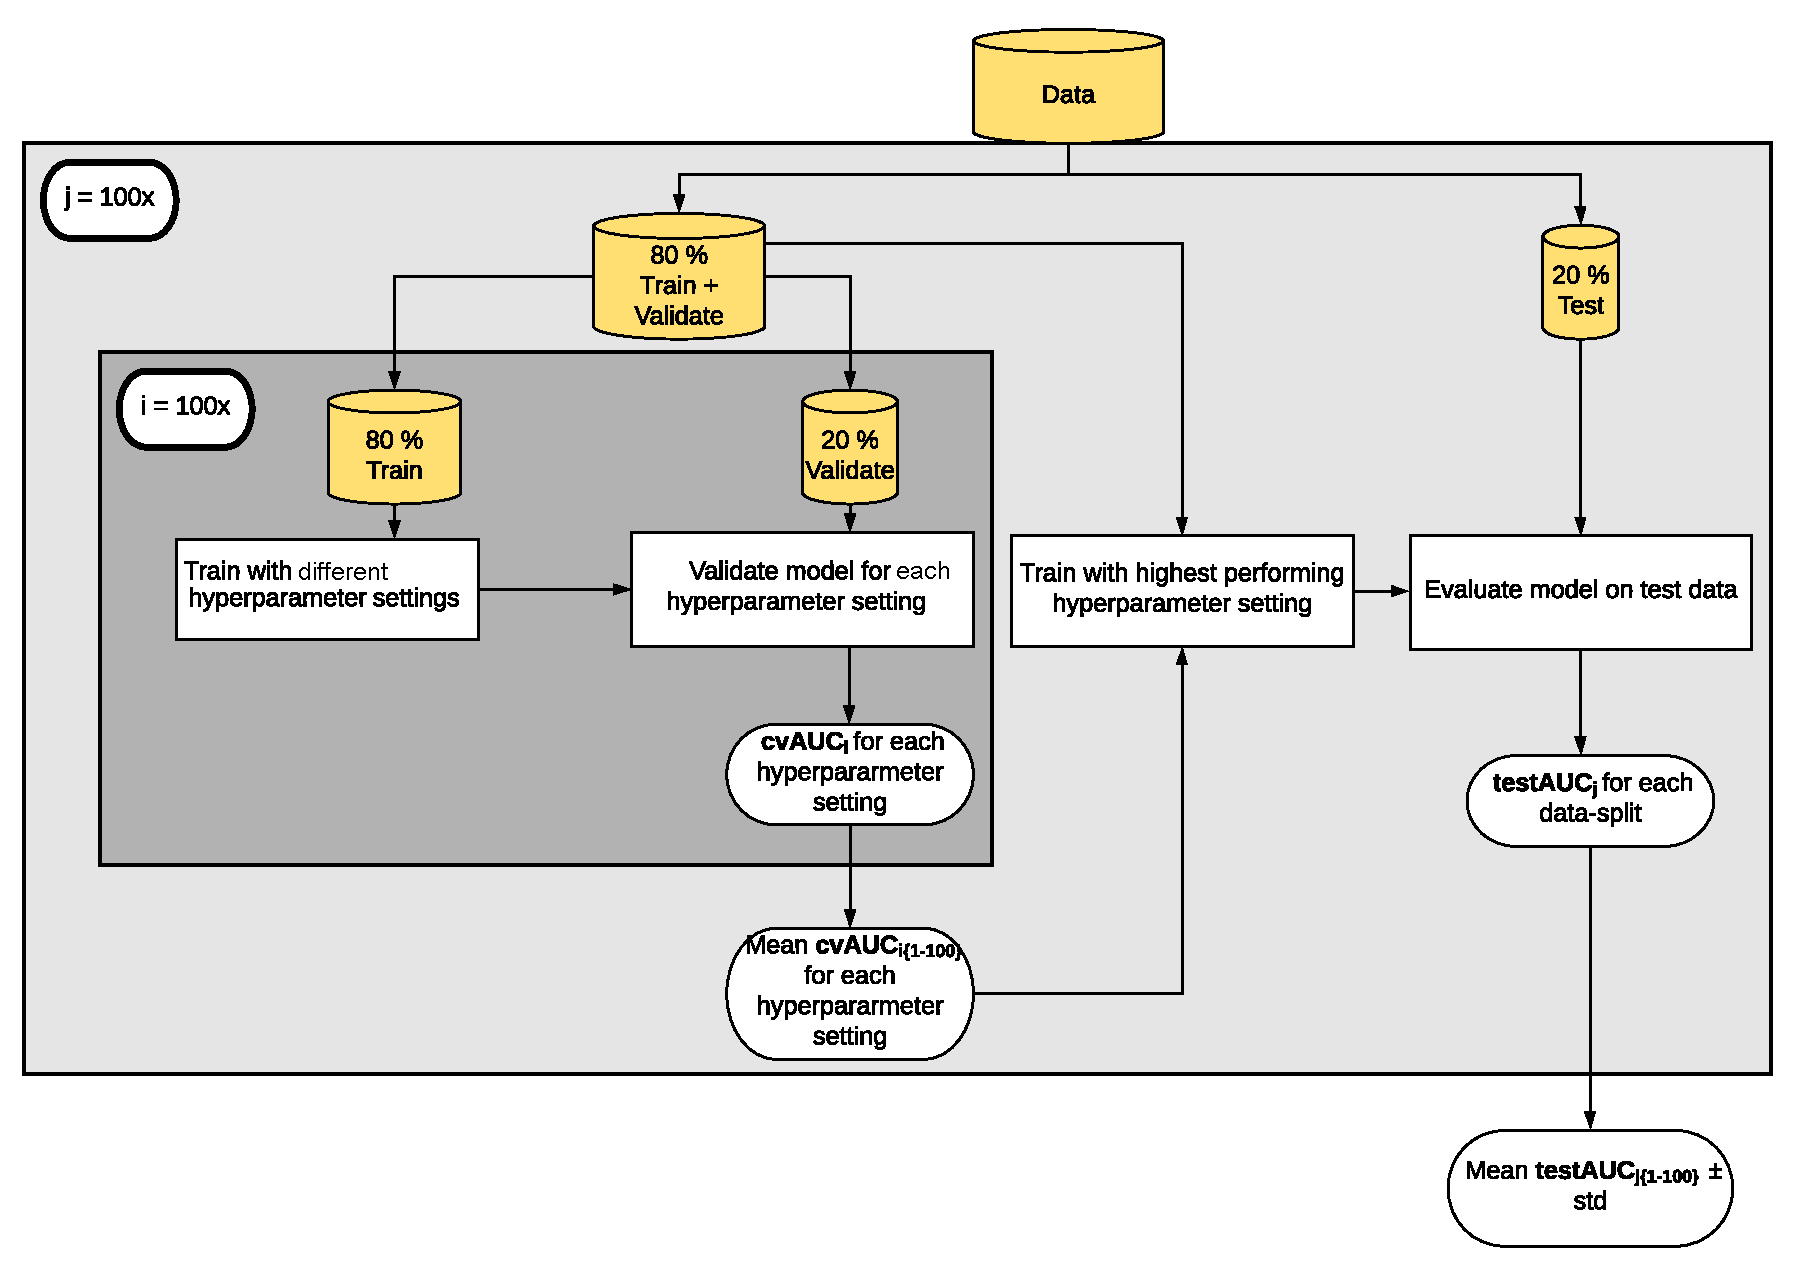
\includegraphics{Figure_1} \textbf{Figure 1. Machine learning pipeline
showing predictive model training and evaluation flowchart. } We split
the data 80\%/20\% stratified to maintain the overall label
distribution, performed five-fold cross-validation on the training data
to select the best hyperparameter setting and then using these
hyperparameters to train all of the training data. The model was
evaluated on a held-out set of data (not used in selecting the model).
Abbreviations: AUROC, area under the receiver operating characteristic
curve \newpage
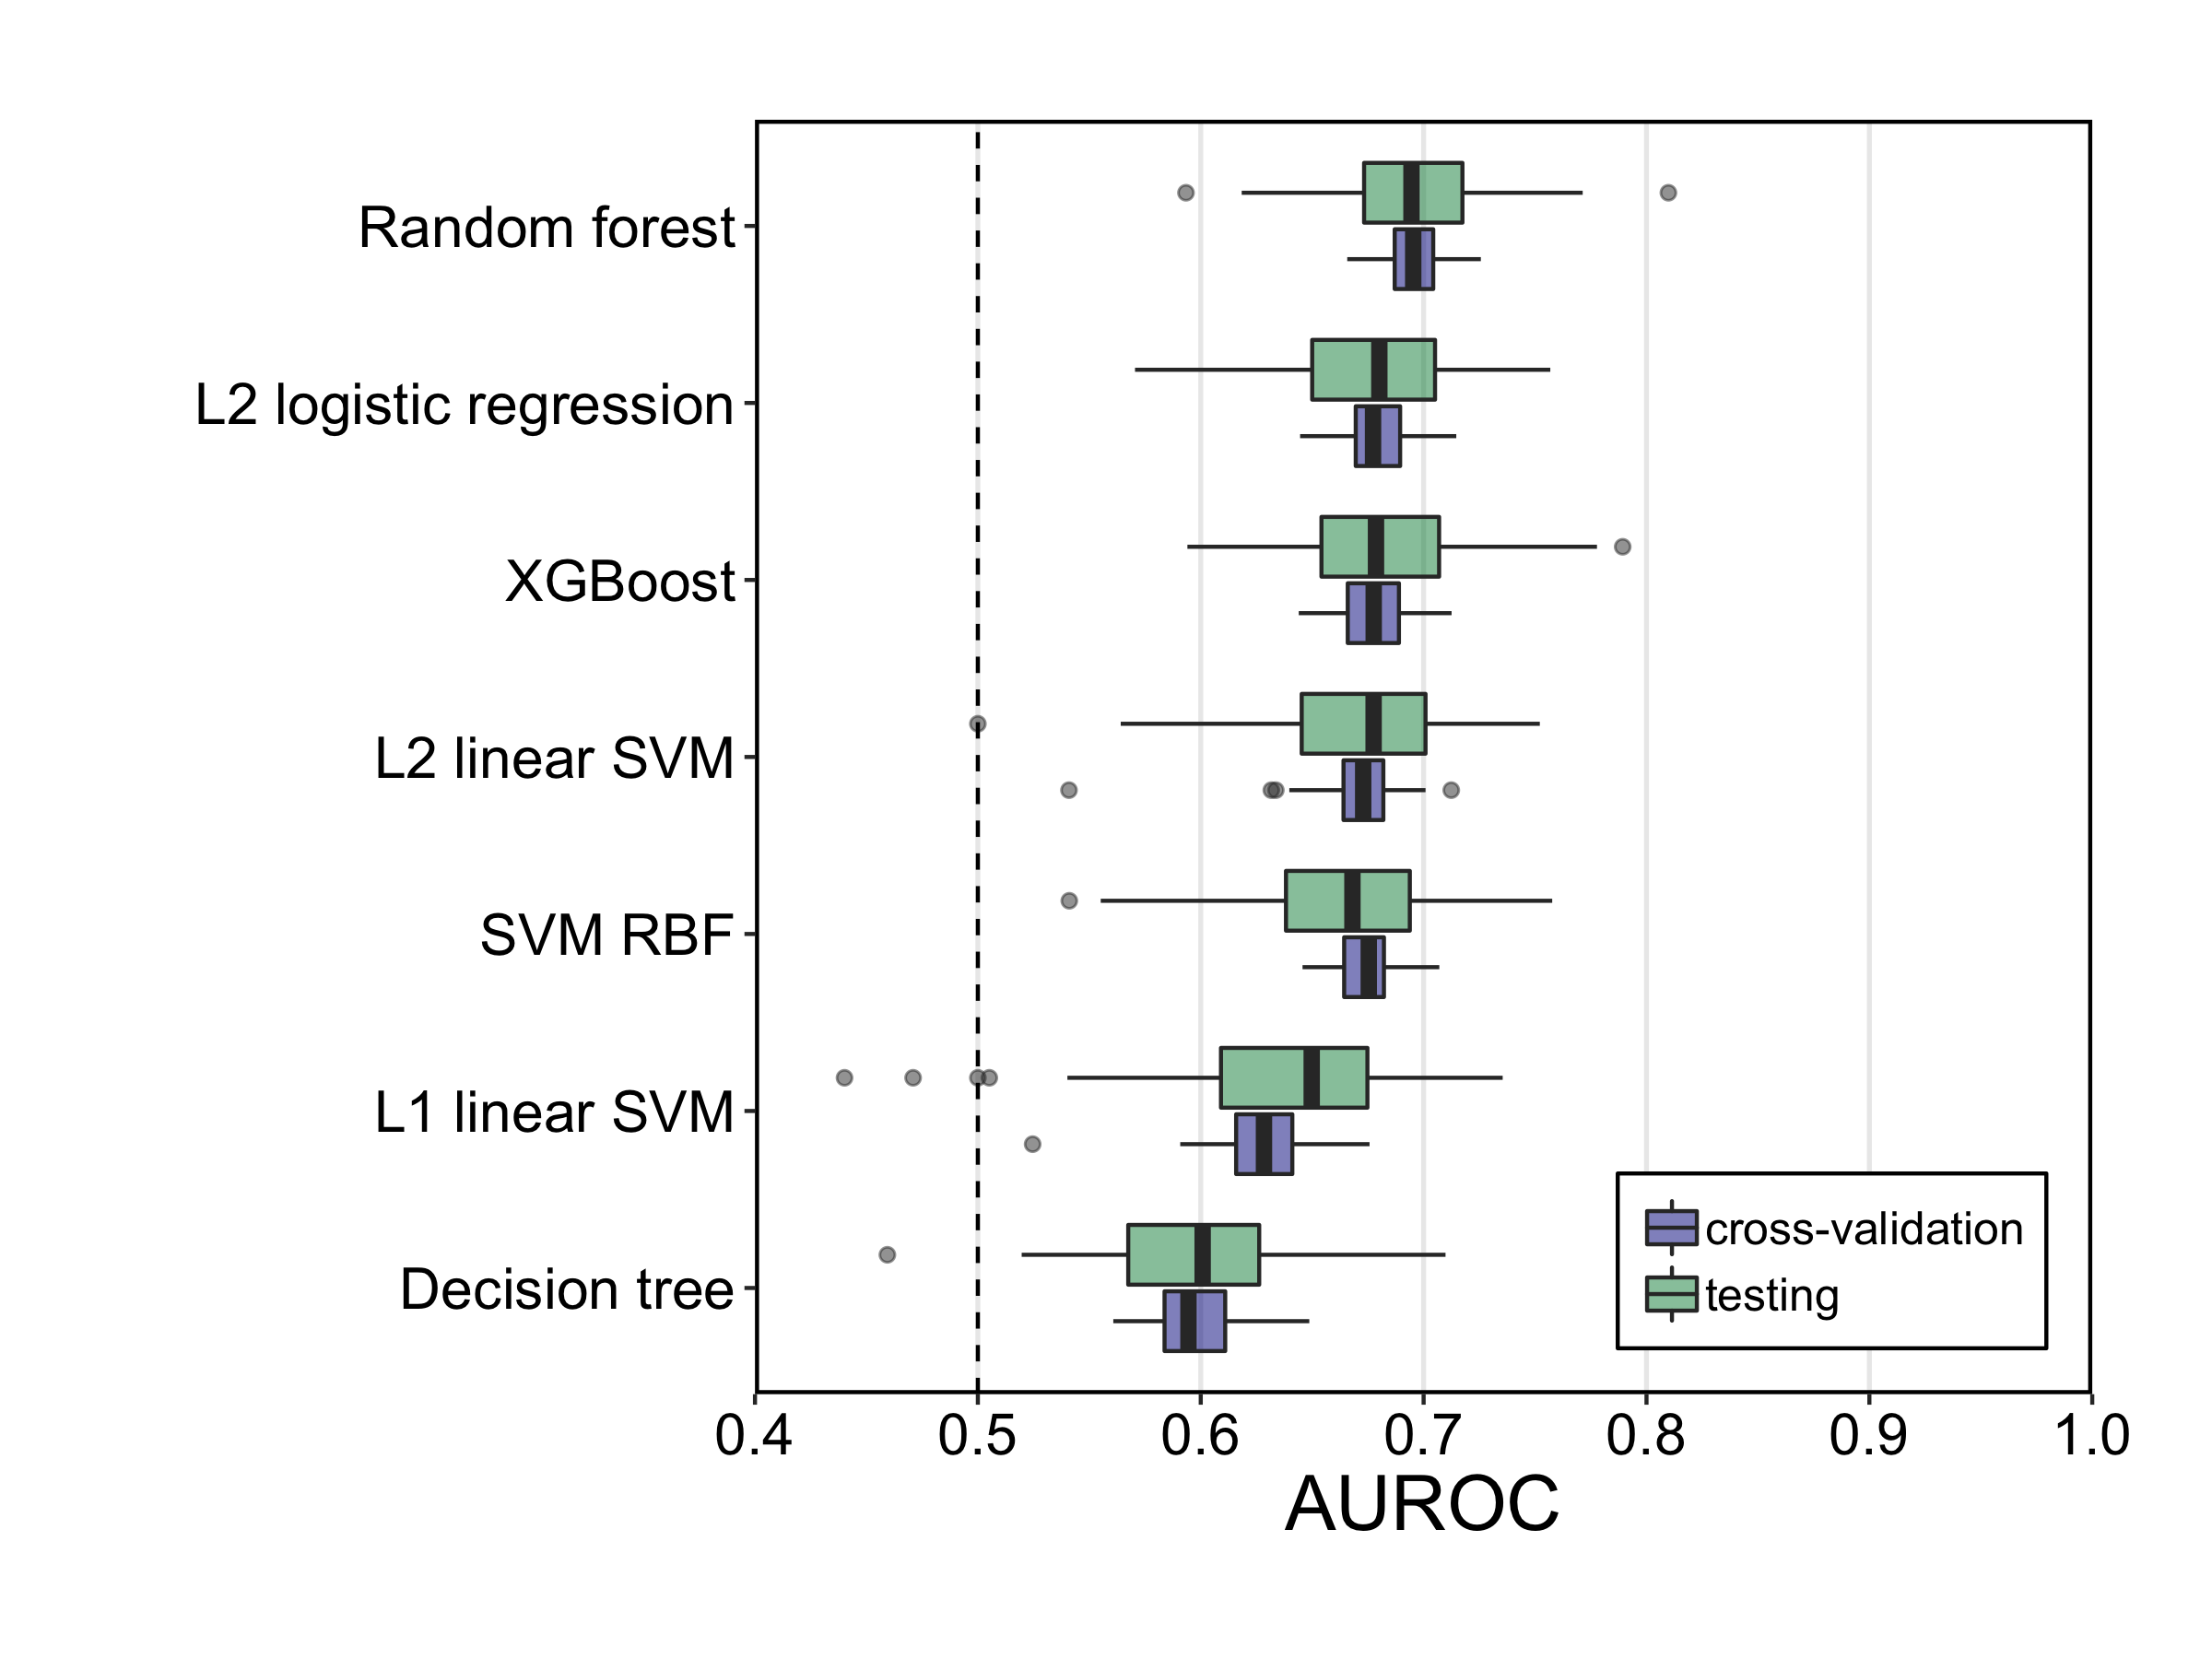
\includegraphics{Figure_2.png} \textbf{Figure 2. Generalization and
classification performance of ML models using AUROC values of all cross
validation and testing performances. } The median AUROC for diagnosing
individuals with SRN using bacterial abundances was higher than chance
(depicted by horizontal line at 0.50) for all the ML models.
Discriminative performance of random forest model was higher than other
ML models. The boxplot shows quartiles at the box ends and the
statistical median as the horizontal line in the box. The whiskers show
the farthest points that are not outliers. Outliers are data points that
are not within 3/2 times the interquartile ranges. Abbreviations: SRN,
screen-relevant neoplasias; AUROC, area under the receiver operating
characteristic curve; SVM, support vector machine; XGBoost, extreme
gradient boosting \newpage
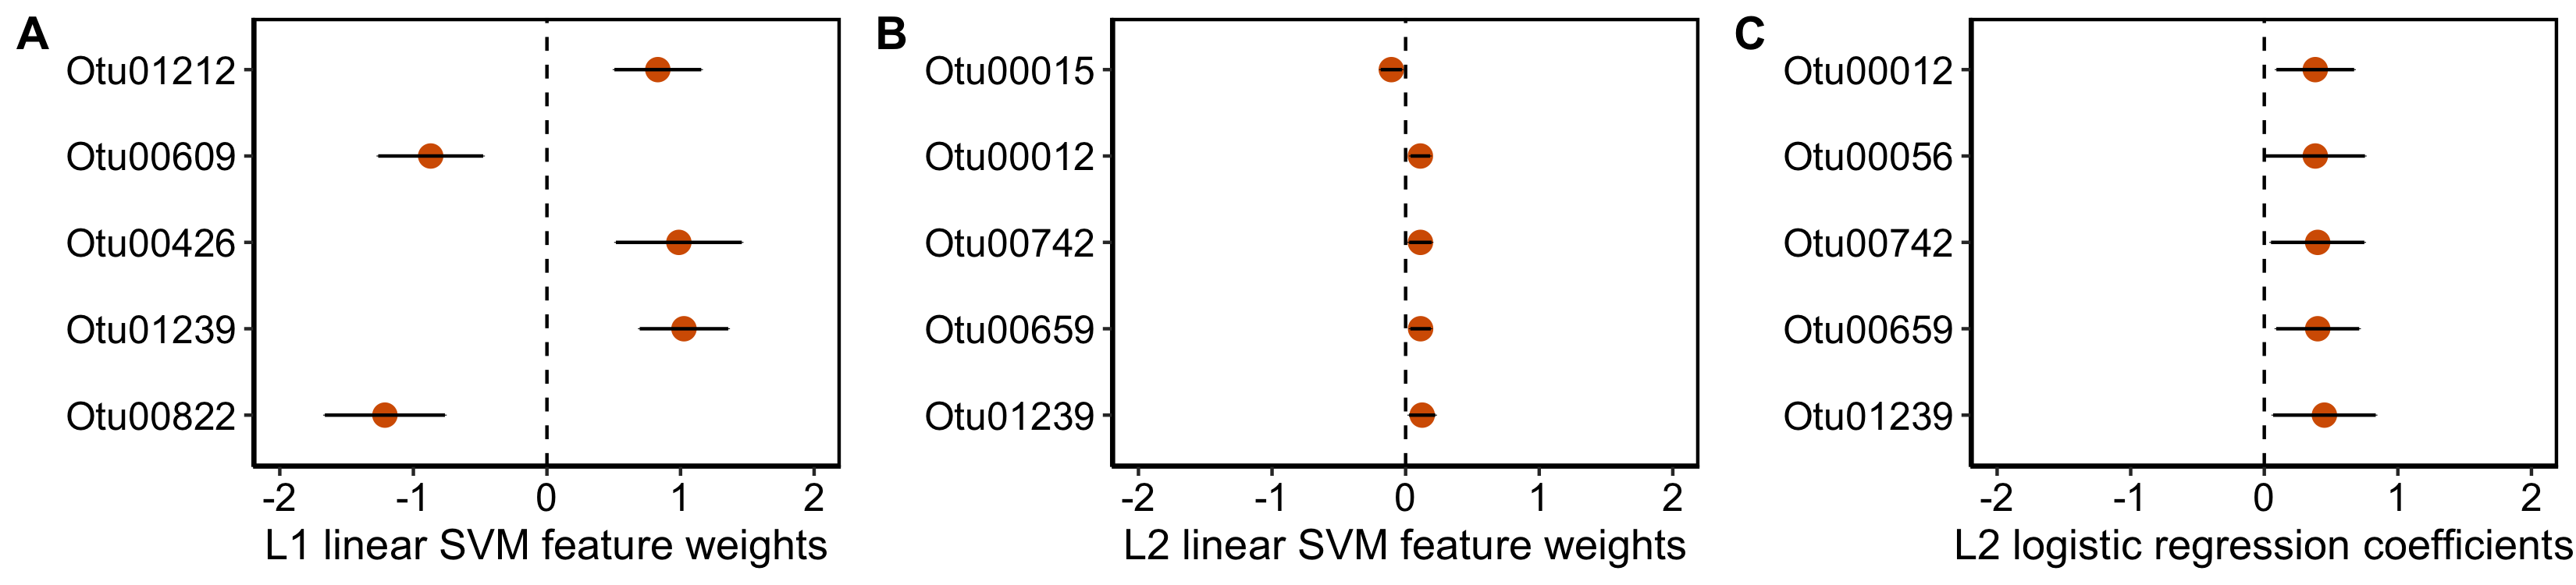
\includegraphics{Figure_3.png} \textbf{Figure 3. Interpretation of the
linear ML models.} (A) L2 logistic regression coefficients (B) L1 SVM
with linear kernel feature weights (C) L2 SVM with linear kernel feature
weights. The means weights and coefficients of the most important five
OTUs for each model are shown here with the standard deviation over 100
data-splits. Similar OTUs had the largest impact on the predictive
performance of L2 logistic regression and L2 SVM with linear kernel.
Abbreviations: SVM, support vector machine; OTU, Operational Taxonomic
Unit. \newpage
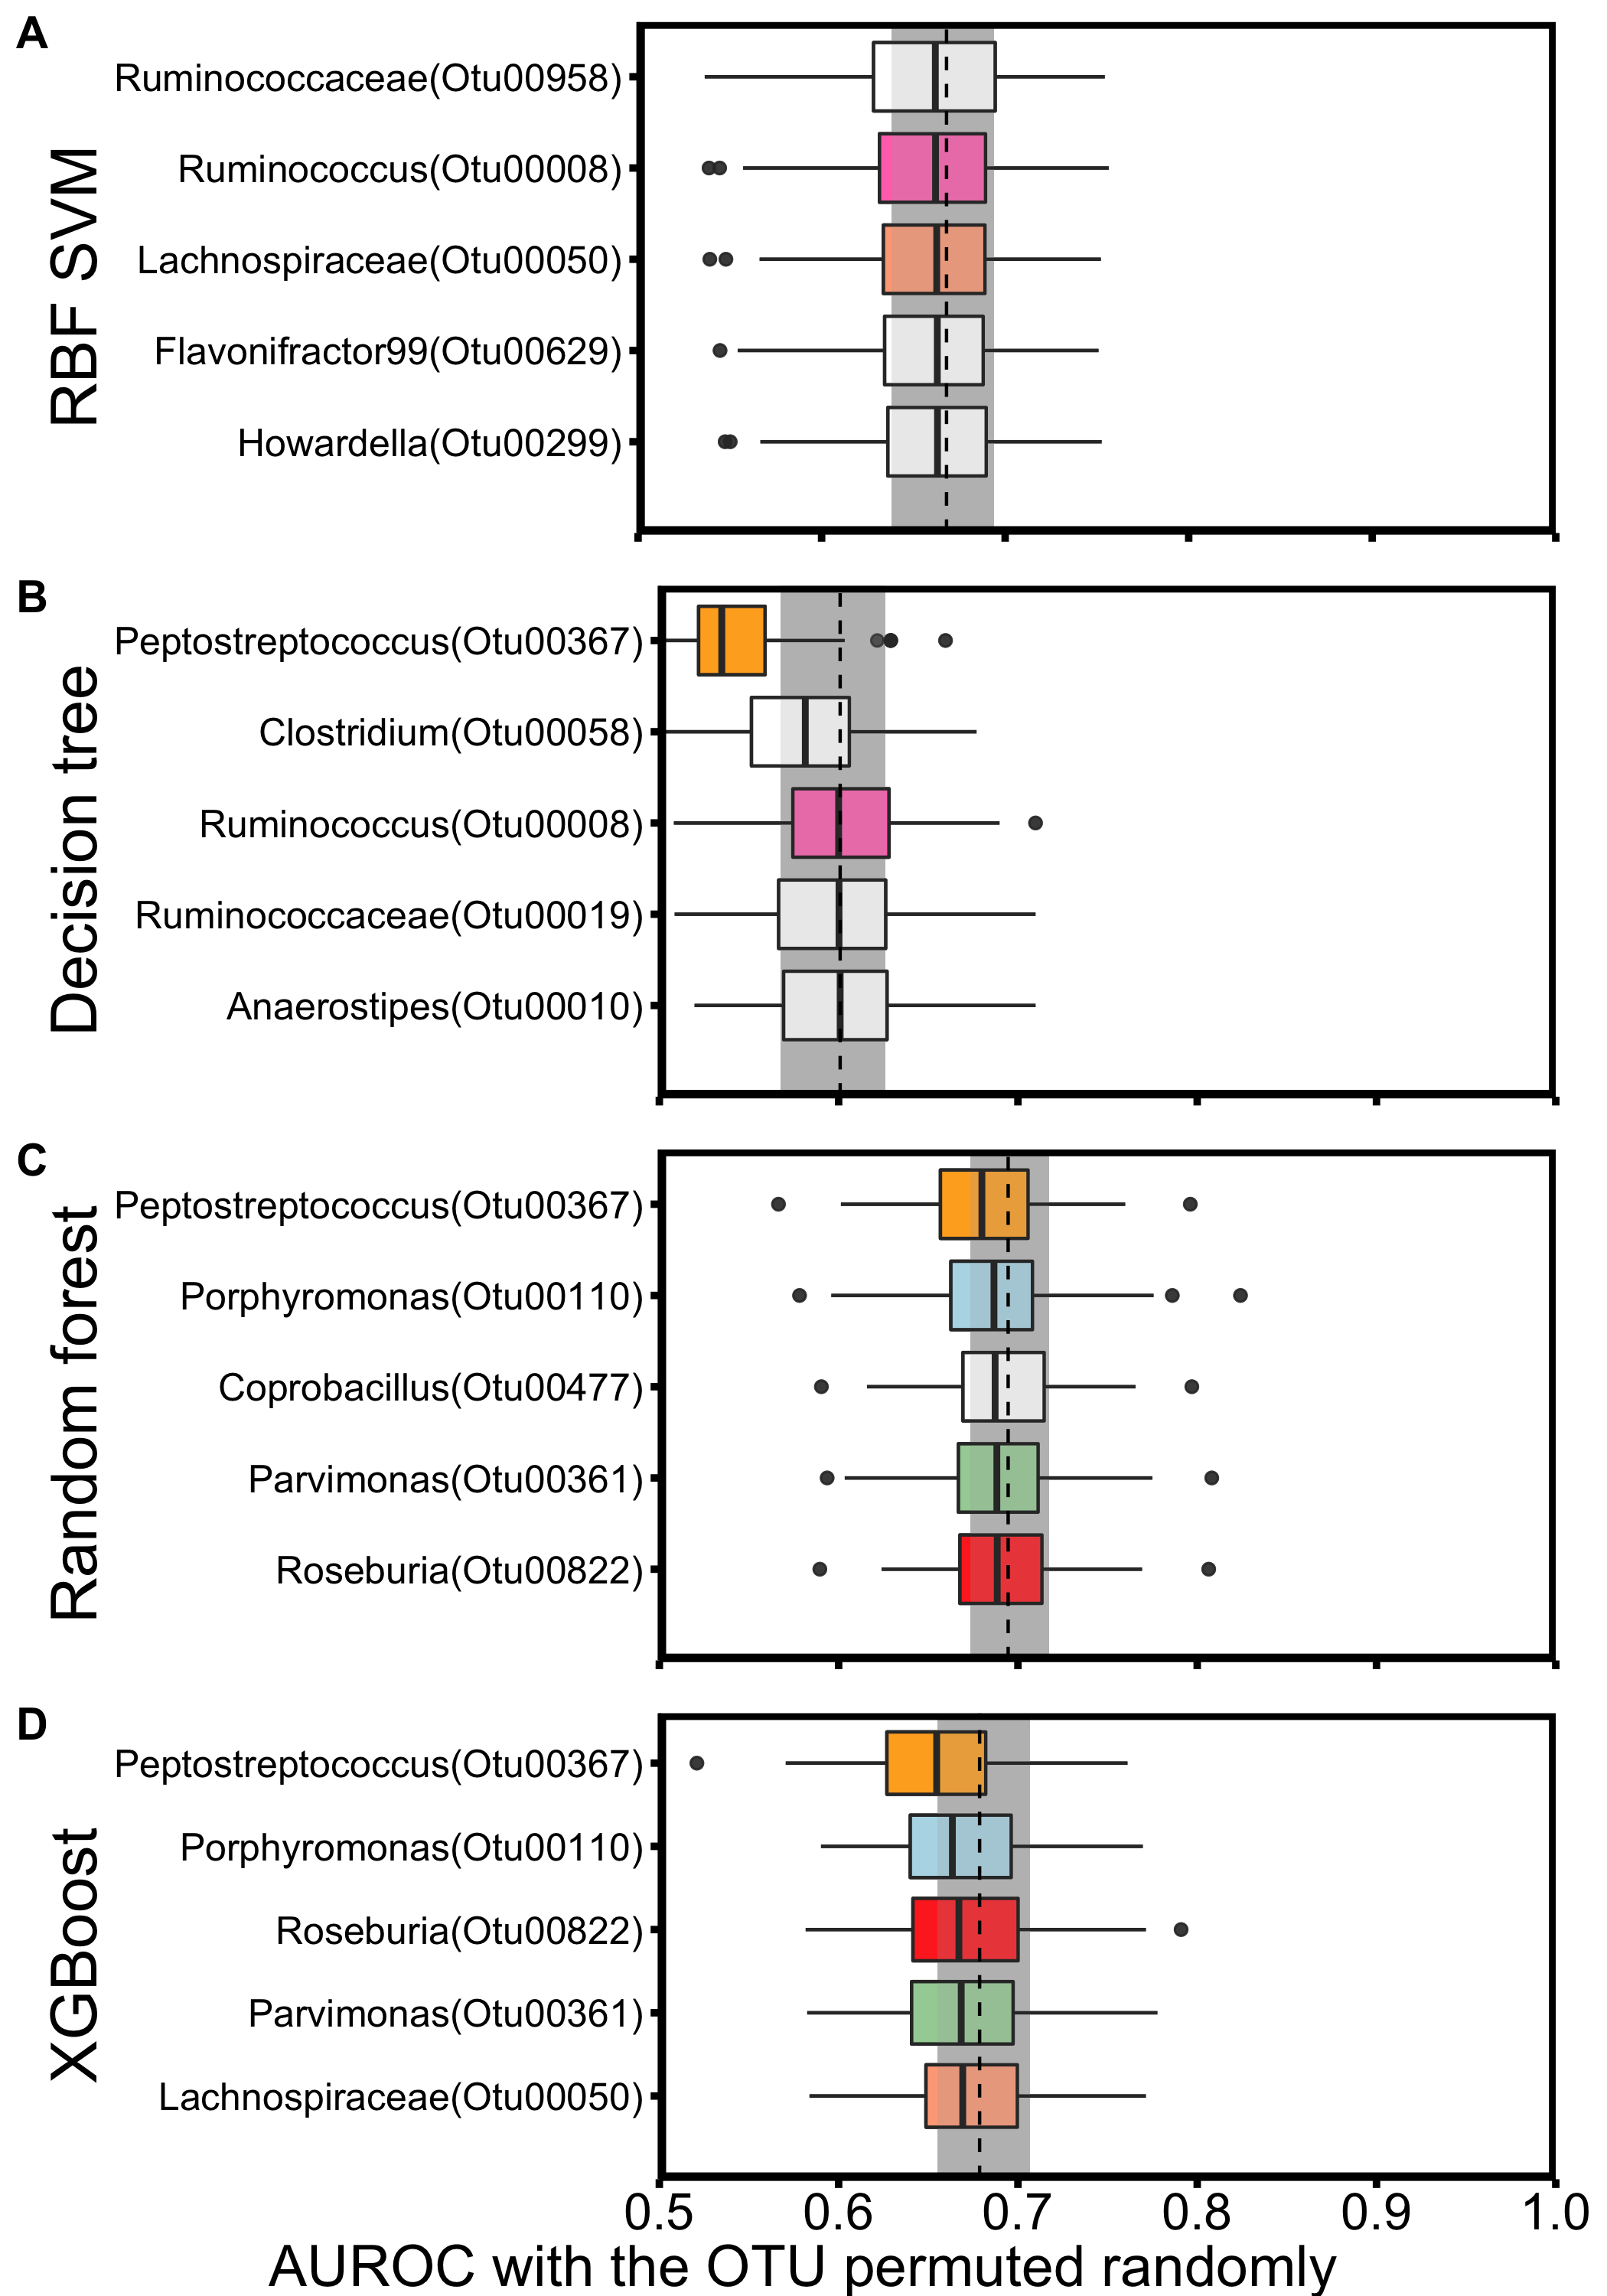
\includegraphics{Figure_4.png} \textbf{Figure 4. Explanation of the
non-linear ML models.} (A) SVM with radial basis kernel (B) decision
tree (C) random forest (D) XGboost feaure importances were explanied
using permutation importance using held-out test set. The gray rectangle
and the dashed line show the IQR range and median of the base testing
AUROC without any permutation performed. For all the tree-based models,
a \emph{Peptostreptococcus} species (OTU00367) had the largest impact on
predictive performance of the model. Abbreviations: SVM, support vector
machine; OTU, Operational Taxonomic Unit; RBF, radial basis kernel; OTU,
Operational Taxonomic Unit. \newpage
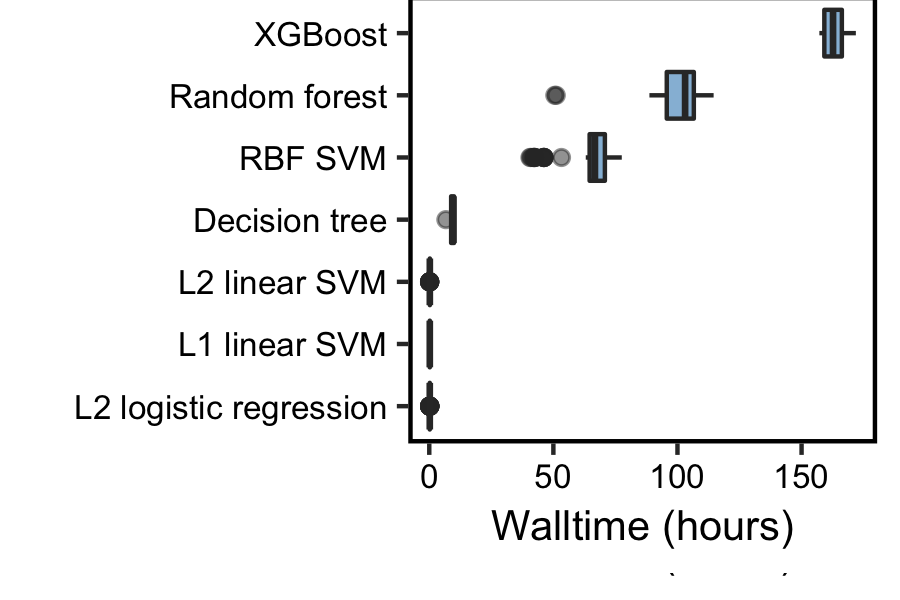
\includegraphics{Figure_5.png} \textbf{Figure 5. Computational
efficiency of seven ML models.} The walltimes for training and testing
of each data-split showed the differences in computational efficieny of
the seven models. The median walltime in hours was the highest for
XGBoost and shortest for L2 logistic regression. The boxplot shows
quartiles at the box ends and the statistical median as the horizontal
line in the box. The whiskers show the farthest points that are not
outliers. Outliers are data points that are not within 3/2 times the
interquartile ranges. Abbreviations: AUROC, area under the receiver
operating characteristic curve; SVM, support vector machine; XGBoost,
extreme gradient boosting.\\
\newpage
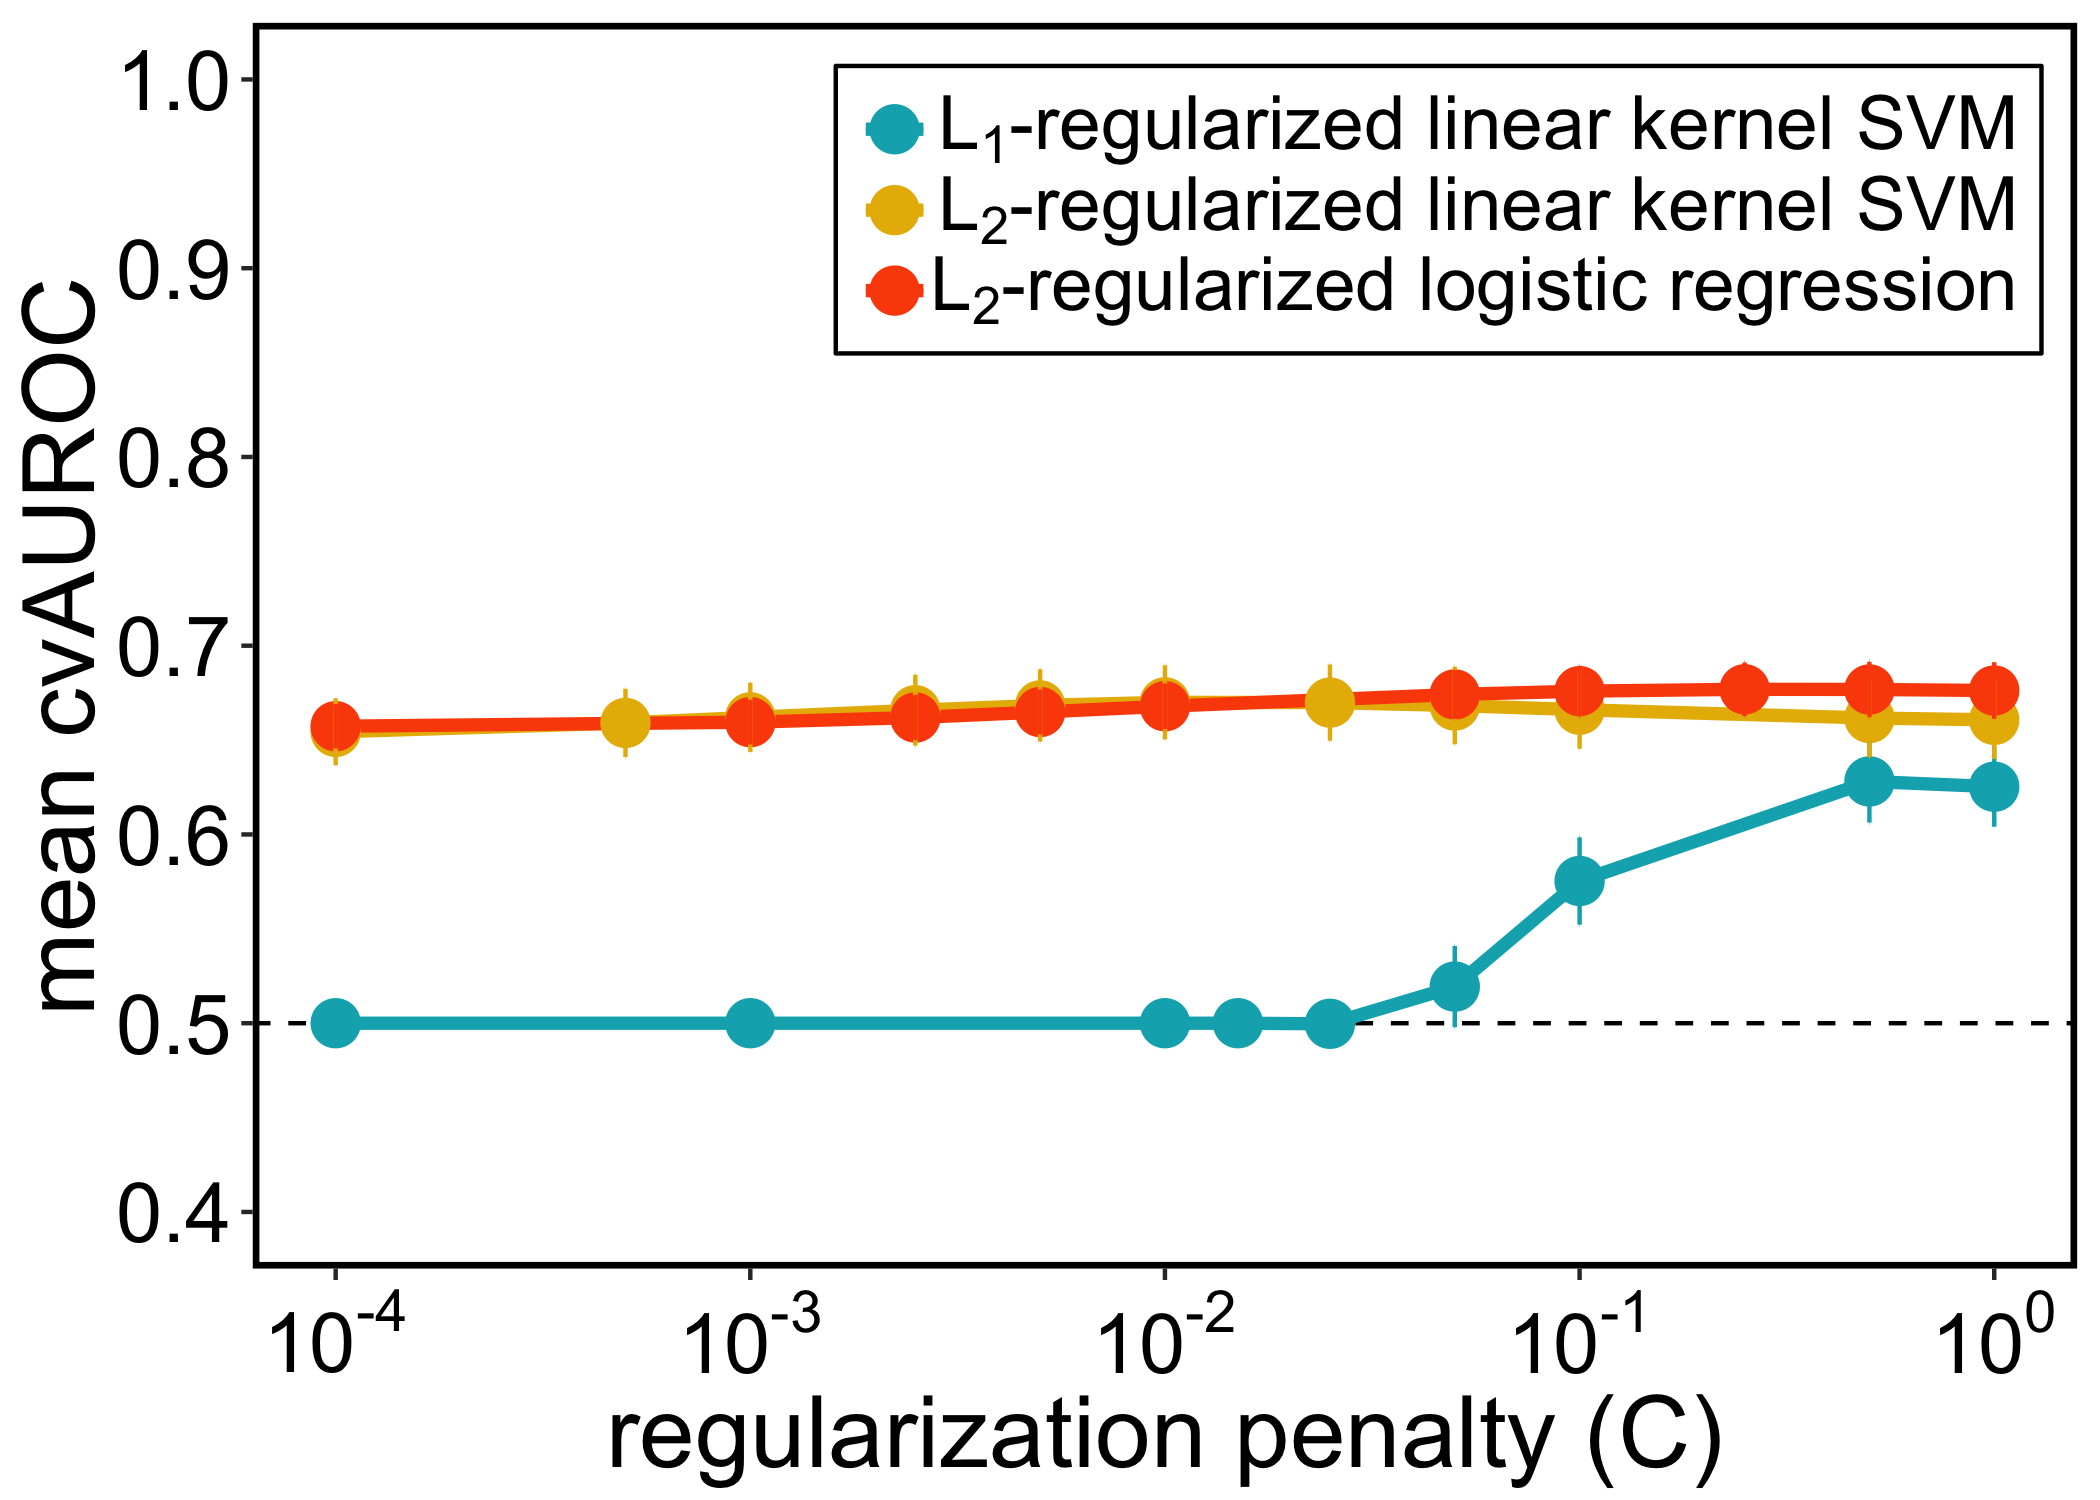
\includegraphics{Figure_S1.png} \textbf{Figure S1. Hyperparameter
setting performances for linear models.} Abbreviations: \newpage
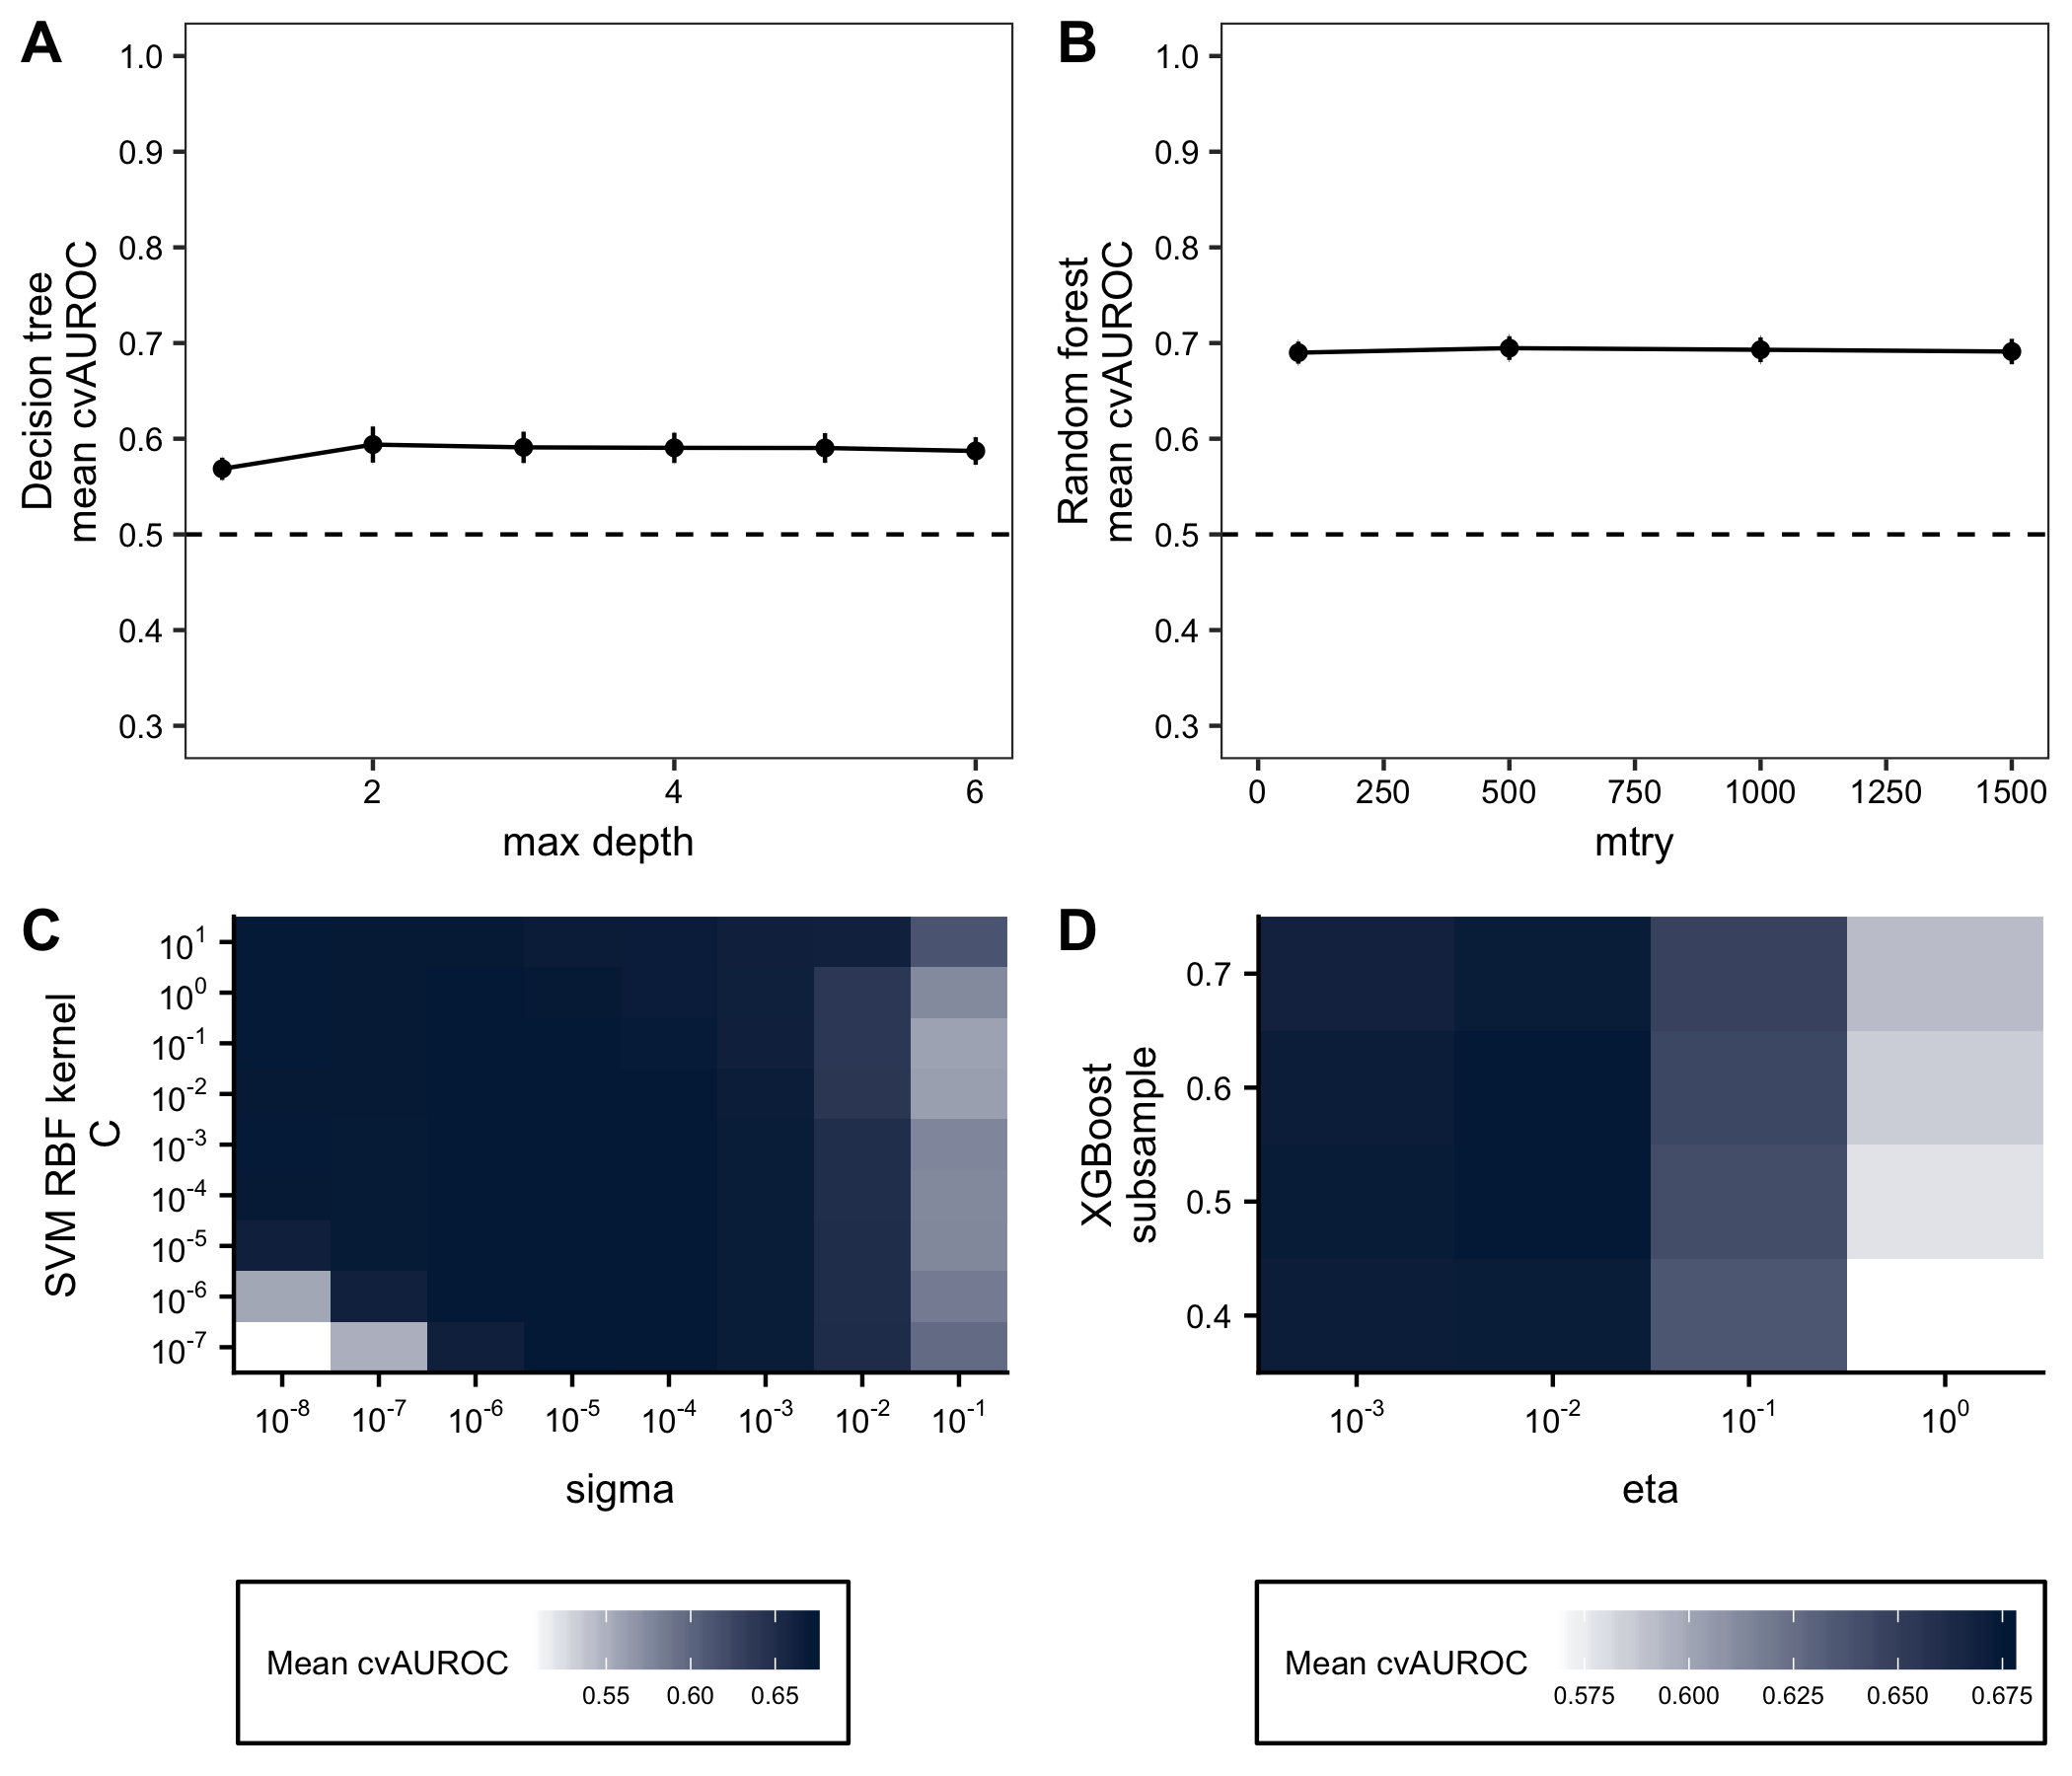
\includegraphics{Figure_S2.png} \textbf{Figure S2. Hyperparameter
setting performances for non-linear models.} Abbreviations: \newpage

\subsection{References}\label{references}

\hypertarget{refs}{}
\hypertarget{ref-zeller_potential_2014}{}
1. \textbf{Zeller G}, \textbf{Tap J}, \textbf{Voigt AY},
\textbf{Sunagawa S}, \textbf{Kultima JR}, \textbf{Costea PI},
\textbf{Amiot A}, \textbf{Böhm J}, \textbf{Brunetti F},
\textbf{Habermann N}, \textbf{Hercog R}, \textbf{Koch M},
\textbf{Luciani A}, \textbf{Mende DR}, \textbf{Schneider MA},
\textbf{Schrotz-King P}, \textbf{Tournigand C}, \textbf{Tran Van Nhieu
J}, \textbf{Yamada T}, \textbf{Zimmermann J}, \textbf{Benes V},
\textbf{Kloor M}, \textbf{Ulrich CM}, \textbf{Knebel Doeberitz M von},
\textbf{Sobhani I}, \textbf{Bork P}. 2014. Potential of fecal microbiota
for early-stage detection of colorectal cancer. Mol Syst Biol
\textbf{10}.
doi:\href{https://doi.org/10.15252/msb.20145645}{10.15252/msb.20145645}.

\hypertarget{ref-zackular_human_2014}{}
2. \textbf{Zackular JP}, \textbf{Rogers MAM}, \textbf{Ruffin MT},
\textbf{Schloss PD}. 2014. The human gut microbiome as a screening tool
for colorectal cancer. Cancer Prev Res \textbf{7}:1112--1121.
doi:\href{https://doi.org/10.1158/1940-6207.CAPR-14-0129}{10.1158/1940-6207.CAPR-14-0129}.

\hypertarget{ref-baxter_dna_2016}{}
3. \textbf{Baxter NT}, \textbf{Koumpouras CC}, \textbf{Rogers MAM},
\textbf{Ruffin MT}, \textbf{Schloss PD}. 2016. DNA from fecal
immunochemical test can replace stool for detection of colonic lesions
using a microbiota-based model. Microbiome \textbf{4}.
doi:\href{https://doi.org/10.1186/s40168-016-0205-y}{10.1186/s40168-016-0205-y}.

\hypertarget{ref-baxter_microbiota-based_2016}{}
4. \textbf{Baxter NT}, \textbf{Ruffin MT}, \textbf{Rogers MAM},
\textbf{Schloss PD}. 2016. Microbiota-based model improves the
sensitivity of fecal immunochemical test for detecting colonic lesions.
Genome Medicine \textbf{8}:37.
doi:\href{https://doi.org/10.1186/s13073-016-0290-3}{10.1186/s13073-016-0290-3}.

\hypertarget{ref-hale_shifts_2017}{}
5. \textbf{Hale VL}, \textbf{Chen J}, \textbf{Johnson S},
\textbf{Harrington SC}, \textbf{Yab TC}, \textbf{Smyrk TC},
\textbf{Nelson H}, \textbf{Boardman LA}, \textbf{Druliner BR},
\textbf{Levin TR}, \textbf{Rex DK}, \textbf{Ahnen DJ}, \textbf{Lance P},
\textbf{Ahlquist DA}, \textbf{Chia N}. 2017. Shifts in the fecal
microbiota associated with adenomatous polyps. Cancer Epidemiol
Biomarkers Prev \textbf{26}:85--94.
doi:\href{https://doi.org/10.1158/1055-9965.EPI-16-0337}{10.1158/1055-9965.EPI-16-0337}.

\hypertarget{ref-pasolli_machine_2016}{}
6. \textbf{Pasolli E}, \textbf{Truong DT}, \textbf{Malik F},
\textbf{Waldron L}, \textbf{Segata N}. 2016. Machine learning
meta-analysis of large metagenomic datasets: Tools and biological
insights. PLoS Comput Biol \textbf{12}.
doi:\href{https://doi.org/10.1371/journal.pcbi.1004977}{10.1371/journal.pcbi.1004977}.

\hypertarget{ref-sze_looking_2016}{}
7. \textbf{Sze MA}, \textbf{Schloss PD}. 2016. Looking for a signal in
the noise: Revisiting obesity and the microbiome. mBio \textbf{7}.
doi:\href{https://doi.org/10.1128/mBio.01018-16}{10.1128/mBio.01018-16}.

\hypertarget{ref-walters_meta-analyses_2014}{}
8. \textbf{Walters WA}, \textbf{Xu Z}, \textbf{Knight R}. 2014.
Meta-analyses of human gut microbes associated with obesity and IBD.
FEBS Lett \textbf{588}:4223--4233.
doi:\href{https://doi.org/10.1016/j.febslet.2014.09.039}{10.1016/j.febslet.2014.09.039}.

\hypertarget{ref-vazquez-baeza_guiding_2018}{}
9. \textbf{Vázquez-Baeza Y}, \textbf{Gonzalez A}, \textbf{Xu ZZ},
\textbf{Washburne A}, \textbf{Herfarth HH}, \textbf{Sartor RB},
\textbf{Knight R}. 2018. Guiding longitudinal sampling in IBD cohorts.
Gut \textbf{67}:1743--1745.
doi:\href{https://doi.org/10.1136/gutjnl-2017-315352}{10.1136/gutjnl-2017-315352}.

\hypertarget{ref-qin_alterations_2014}{}
10. \textbf{Qin N}, \textbf{Yang F}, \textbf{Li A}, \textbf{Prifti E},
\textbf{Chen Y}, \textbf{Shao L}, \textbf{Guo J}, \textbf{Le Chatelier
E}, \textbf{Yao J}, \textbf{Wu L}, \textbf{Zhou J}, \textbf{Ni S},
\textbf{Liu L}, \textbf{Pons N}, \textbf{Batto JM}, \textbf{Kennedy SP},
\textbf{Leonard P}, \textbf{Yuan C}, \textbf{Ding W}, \textbf{Chen Y},
\textbf{Hu X}, \textbf{Zheng B}, \textbf{Qian G}, \textbf{Xu W},
\textbf{Ehrlich SD}, \textbf{Zheng S}, \textbf{Li L}. 2014. Alterations
of the human gut microbiome in liver cirrhosis. Nature
\textbf{513}:59--64.
doi:\href{https://doi.org/10.1038/nature13568}{10.1038/nature13568}.

\hypertarget{ref-geman_deep_2018}{}
11. \textbf{Geman O}, \textbf{Chiuchisan I}, \textbf{Covasa M},
\textbf{Doloc C}, \textbf{Milici M-R}, \textbf{Milici L-D}. 2018. Deep
learning tools for human microbiome big data, pp. 265--275. \emph{In}
Balas, VE, Jain, LC, Balas, MM (eds.), Soft computing applications.
Springer International Publishing.

\hypertarget{ref-thaiss_persistent_2016}{}
12. \textbf{Thaiss CA}, \textbf{Itav S}, \textbf{Rothschild D},
\textbf{Meijer MT}, \textbf{Levy M}, \textbf{Moresi C},
\textbf{Dohnalová L}, \textbf{Braverman S}, \textbf{Rozin S},
\textbf{Malitsky S}, \textbf{Dori-Bachash M}, \textbf{Kuperman Y},
\textbf{Biton I}, \textbf{Gertler A}, \textbf{Harmelin A},
\textbf{Shapiro H}, \textbf{Halpern Z}, \textbf{Aharoni A},
\textbf{Segal E}, \textbf{Elinav E}. 2016. Persistent microbiome
alterations modulate the rate of post-dieting weight regain. Nature
\textbf{540}:544--551.
doi:\href{https://doi.org/10.1038/nature20796}{10.1038/nature20796}.

\hypertarget{ref-flemer_oral_2018}{}
13. \textbf{Flemer B}, \textbf{Warren RD}, \textbf{Barrett MP},
\textbf{Cisek K}, \textbf{Das A}, \textbf{Jeffery IB}, \textbf{Hurley
E}, \textbf{O`Riordain M}, \textbf{Shanahan F}, \textbf{O`Toole PW}.
2018. The oral microbiota in colorectal cancer is distinctive and
predictive. Gut \textbf{67}:1454--1463.
doi:\href{https://doi.org/10.1136/gutjnl-2017-314814}{10.1136/gutjnl-2017-314814}.

\hypertarget{ref-dai_multi-cohort_2018}{}
14. \textbf{Dai Z}, \textbf{Coker OO}, \textbf{Nakatsu G}, \textbf{Wu
WKK}, \textbf{Zhao L}, \textbf{Chen Z}, \textbf{Chan FKL},
\textbf{Kristiansen K}, \textbf{Sung JJY}, \textbf{Wong SH}, \textbf{Yu
J}. 2018. Multi-cohort analysis of colorectal cancer metagenome
identified altered bacteria across populations and universal bacterial
markers. Microbiome \textbf{6}:70.
doi:\href{https://doi.org/10.1186/s40168-018-0451-2}{10.1186/s40168-018-0451-2}.

\hypertarget{ref-montassier_pretreatment_2016}{}
15. \textbf{Montassier E}, \textbf{Al-Ghalith GA}, \textbf{Ward T},
\textbf{Corvec S}, \textbf{Gastinne T}, \textbf{Potel G}, \textbf{Moreau
P}, \textbf{Cochetiere MF de la}, \textbf{Batard E}, \textbf{Knights D}.
2016. Pretreatment gut microbiome predicts chemotherapy-related
bloodstream infection. Genome Medicine \textbf{8}:49.
doi:\href{https://doi.org/10.1186/s13073-016-0301-4}{10.1186/s13073-016-0301-4}.

\hypertarget{ref-papa_non-invasive_2012}{}
16. \textbf{Papa E}, \textbf{Docktor M}, \textbf{Smillie C},
\textbf{Weber S}, \textbf{Preheim SP}, \textbf{Gevers D},
\textbf{Giannoukos G}, \textbf{Ciulla D}, \textbf{Tabbaa D},
\textbf{Ingram J}, \textbf{Schauer DB}, \textbf{Ward DV},
\textbf{Korzenik JR}, \textbf{Xavier RJ}, \textbf{Bousvaros A},
\textbf{Alm EJ}. 2012. Non-invasive mapping of the gastrointestinal
microbiota identifies children with inflammatory bowel disease. PLOS ONE
\textbf{7}:e39242.
doi:\href{https://doi.org/10.1371/journal.pone.0039242}{10.1371/journal.pone.0039242}.

\hypertarget{ref-mossotto_classification_2017}{}
17. \textbf{Mossotto E}, \textbf{Ashton JJ}, \textbf{Coelho T},
\textbf{Beattie RM}, \textbf{MacArthur BD}, \textbf{Ennis S}. 2017.
Classification of paediatric inflammatory bowel disease using machine
learning. Scientific Reports \textbf{7}.
doi:\href{https://doi.org/10.1038/s41598-017-02606-2}{10.1038/s41598-017-02606-2}.

\hypertarget{ref-ai_systematic_2017}{}
18. \textbf{Ai L}, \textbf{Tian H}, \textbf{Chen Z}, \textbf{Chen H},
\textbf{Xu J}, \textbf{Fang J-Y}. 2017. Systematic evaluation of
supervised classifiers for fecal microbiota-based prediction of
colorectal cancer. Oncotarget \textbf{8}:9546--9556.
doi:\href{https://doi.org/10.18632/oncotarget.14488}{10.18632/oncotarget.14488}.

\hypertarget{ref-wong_quantitation_2017}{}
19. \textbf{Wong SH}, \textbf{Kwong TNY}, \textbf{Chow T-C}, \textbf{Luk
AKC}, \textbf{Dai RZW}, \textbf{Nakatsu G}, \textbf{Lam TYT},
\textbf{Zhang L}, \textbf{Wu JCY}, \textbf{Chan FKL}, \textbf{Ng SSM},
\textbf{Wong MCS}, \textbf{Ng SC}, \textbf{Wu WKK}, \textbf{Yu J},
\textbf{Sung JJY}. 2017. Quantitation of faecal fusobacterium improves
faecal immunochemical test in detecting advanced colorectal neoplasia.
Gut \textbf{66}:1441--1448.
doi:\href{https://doi.org/10.1136/gutjnl-2016-312766}{10.1136/gutjnl-2016-312766}.

\hypertarget{ref-galkin_human_2018}{}
20. \textbf{Galkin F}, \textbf{Aliper A}, \textbf{Putin E},
\textbf{Kuznetsov I}, \textbf{Gladyshev VN}, \textbf{Zhavoronkov A}.
2018. Human microbiome aging clocks based on deep learning and tandem of
permutation feature importance and accumulated local effects. bioRxiv.
doi:\href{https://doi.org/10.1101/507780}{10.1101/507780}.

\hypertarget{ref-reiman_using_2017}{}
21. \textbf{Reiman D}, \textbf{Metwally A}, \textbf{Dai Y}. 2017. Using
convolutional neural networks to explore the microbiome, pp. 4269--4272.
\emph{In} 2017 39th annual international conference of the IEEE
engineering in medicine and biology society (EMBC).

\hypertarget{ref-fioravanti_phylogenetic_2017}{}
22. \textbf{Fioravanti D}, \textbf{Giarratano Y}, \textbf{Maggio V},
\textbf{Agostinelli C}, \textbf{Chierici M}, \textbf{Jurman G},
\textbf{Furlanello C}. 2017. Phylogenetic convolutional neural networks
in metagenomics. arXiv:170902268 {[}cs, q-bio{]}.

\hypertarget{ref-sze_leveraging_2018}{}
23. \textbf{Sze MA}, \textbf{Schloss PD}. 2018. Leveraging existing 16S
rRNA gene surveys to identify reproducible biomarkers in individuals
with colorectal tumors. mBio \textbf{9}:e00630--18.
doi:\href{https://doi.org/10.1128/mBio.00630-18}{10.1128/mBio.00630-18}.

\hypertarget{ref-schloss_introducing_2009}{}
24. \textbf{Schloss PD}, \textbf{Westcott SL}, \textbf{Ryabin T},
\textbf{Hall JR}, \textbf{Hartmann M}, \textbf{Hollister EB},
\textbf{Lesniewski RA}, \textbf{Oakley BB}, \textbf{Parks DH},
\textbf{Robinson CJ}, \textbf{Sahl JW}, \textbf{Stres B},
\textbf{Thallinger GG}, \textbf{Van Horn DJ}, \textbf{Weber CF}. 2009.
Introducing mothur: Open-Source, Platform-Independent,
Community-Supported Software for Describing and Comparing Microbial
Communities. ApplEnvironMicrobiol \textbf{75}:7537--7541.

\hypertarget{ref-westcott_opticlust_2017}{}
25. \textbf{Westcott SL}, \textbf{Schloss PD}. 2017. OptiClust, an
Improved Method for Assigning Amplicon-Based Sequence Data to
Operational Taxonomic Units. mSphere \textbf{2}.
doi:\href{https://doi.org/10.1128/mSphereDirect.00073-17}{10.1128/mSphereDirect.00073-17}.

\hypertarget{ref-rognes_vsearch_2016}{}
26. \textbf{Rognes T}, \textbf{Flouri T}, \textbf{Nichols B},
\textbf{Quince C}, \textbf{Mahé F}. 2016. VSEARCH: A versatile open
source tool for metagenomics. PeerJ \textbf{4}:e2584.
doi:\href{https://doi.org/10.7717/peerj.2584}{10.7717/peerj.2584}.


\end{document}
